\begin{opin}{\guscolor}{Gustavo}

\subsubsection{Emoción y Aprendizaje}

En el día de hoy hemos terminado el tema 02 relacionado con la neurodidáctica y me ha impactado la pregunta que nos ha hecho Raquel en clase porque resume muy bien la relación existente entre emoción y aprendizaje. La pregunta es la siguiente:

\textbf{¿Recuerdas lo que estabas haciendo el 11 de Septiembre de 2001 cuando los aviones se estrellaron contra las torres gemelas de Nueva York?}

Es alucinante como un alto porcentaje de la gente a la que le preguntas recuerda exactamente donde estaba y lo qué estaba haciendo.

Se me ocurre otra pregunta similar: \textbf{¿Recuerdas donde viste a España ganar la Copa del Mundo de Futbol de Sudáfrica 2010?}

Como veis estas emociones pueden ser positivas o negativas. Pero lo importante es que haya emoción.

Estos son claros ejemplos de que si hay emociones, hay aprendizaje. Me atrevería a definirlo como un aprendizaje inconsciente y que permanece en la memoria a largo plazo.

Toda esta relación entre emociones y aprendizaje es aún más importante en la adolescencia porque en esta etapa de la vida el cerebro demanda dopamina. Para liberar la dopamina, se necesitan cosas emocionantes. Por ejemplo, cuando nos divertimos segregamos dopamina. El aprendizaje debe ser divertido. 

\subsubsection{La motivación escolar: siete etapas clave}

Volviendo a lo que no terminamos de determinar la semana pasada. El diagnóstico de la situación está claro. ¿Qué podemos hacer para cambiarlo?

Realizar cambios implicaría cambiar con lo establecido y hay muchas personas que tienen miedo a lo desconocido y por eso deciden no cambiar. Solo hay que ver las fotografías de las transparencias de clase para darse cuenta de que al igual que en otros aspectos la sociedad ha evolucionado, en la educación nos hemos quedado estancados.

\label{noevolucionEdu}

\begin{minipage}[hbtp]{0.9\linewidth}
	
	
	\begin{tabular}{cc}
		\begin{minipage}[hbtp]{0.5\linewidth}
			\centering
			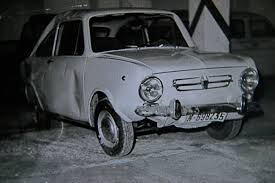
\includegraphics[width=0.8\linewidth]{img/coche1.jpg}
			\captionof{figure}{Coche de mediadios del siglo pasado.}
		\end{minipage}
		&
		\begin{minipage}[hbtp]{0.5\linewidth}
			\centering
			
\includegraphics[width=0.8\linewidth]{img/coche2.jpg}
			\captionof{figure}{Coche actual.}
		\end{minipage}\\
		\begin{minipage}[hbtp]{0.5\linewidth}
			\centering
			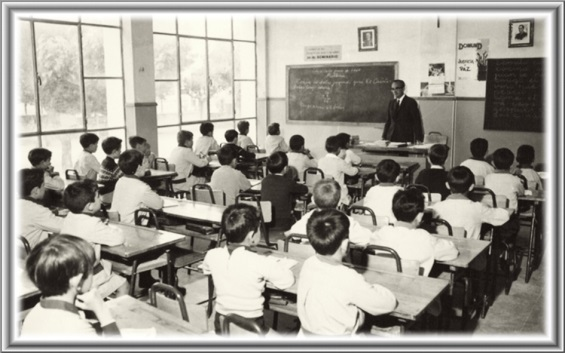
\includegraphics[width=0.8\linewidth]{img/coche3.jpg}
			\captionof{figure}{Educación de mediados del siglo pasado.}
		\end{minipage}
		&
		\begin{minipage}[hbtp]{0.5\linewidth}
			\centering
			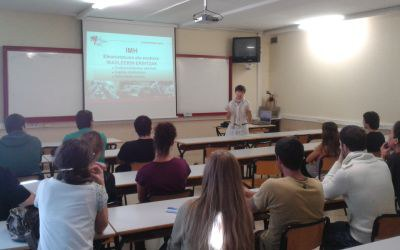
\includegraphics[width=0.8\linewidth]{img/coche4.jpg}
			\captionof{figure}{Educación actual.}
		\end{minipage}
	\end{tabular}
	%\captionof{tabular}{Resumen de la necesidad de innovación en la educación.}
	
\end{minipage}


Para describir cómo podemos cambiar la situación, me voy a basar en el análisis del artículo del blog “Escuela con cerebro” (\href{https://escuelaconcerebro.wordpress.com/2014/09/18/la-motivacion-escolar-siete-etapas-clave/}{https://escuelaconcerebro.wordpress.com/2014/09/18/la-motivacion-escolar-siete-etapas-clave/}) en el que nos hace pensar acerca de lo que podemos hacer en la práctica los profesores para motivar al alumno, cómo conseguir despertar su interés por el aprendizaje (motivación inicial), mantener una implicación regular (motivación de logro) o hacer que el proceso de evaluación sea útil, entre otras cosas.

Analizando las etapas clave

\paragraph{1. Qué curioso}

En los inicios de clase o de las unidades didácticas correspondientes es imprescindible hacer presentaciones activas y variadas que pueden alternar visualizaciones de videos, planteamientos de preguntas al modo socrático clásico, utilización de anécdotas o ejemplos adecuados, etc.

Considero muy importante despertar el interés del alumno a la hora de afrontar un nuevo reto.

\paragraph{2. ¡Esto me interesa!}

Cuando los contenidos que se van a trabajar son contenidos reales cercanos a la vida del alumno y con un enfoque interdisciplinar es más fácil que se motive.

Hay poco que explicar acerca de esta etapa. Puede ser complicado buscar motivaciones individuales para cada alumno, aunque este sería el caso óptimo.

\paragraph{3. ¡Acepto el reto!}

Para no desmotivar al alumnado, los retos han de ser adecuados para que no se sientan cómodos, pero que tampoco se depriman porque les parezcan muy difíciles de abordar.

\paragraph{4. ¡Soy el protagonista!}

Hemos de respetar las preguntas, intervenciones, debates suscitados o análisis entre alumnos sin prisas (no hay excusas con lo de acabar el temario; lo importante no es lo que enseñamos sino lo que aprenden) y permitirles que intervengan en la creación de normas, elección de problemas o estrategias de trabajo.

Me encanta esta afirmación dado que muchas veces, el miedo o vergüenza a ser rechazado por preguntar cosas que deberían saber hace que muchos alumnos se queden estancados y pierdan el interés por la materia.

Esto pasa también en los entornos laborales y no ayudan para nada en el aprendizaje colaborativo.

\paragraph{5. ¡Progreso!}

La memoria es esencial para el aprendizaje (de hecho son dos procesos indisolubles) y lo que ocurre es que hay que hacer un uso adecuado de ella en cada tarea. Para que el progreso del alumno sea real se ha de poder integrar la nueva información con la ya conocida.

Puede parecer que solo queremos que los alumnos aprendan a base de juegos y emociones y acercarles las materias a cosas reales que ellos pueden relacionar. Sin embargo no hay que olvidar que es imposible no retener nada en la memoria. El ejemplo de saberse las tablas de multiplicación es muy descriptivo.

\paragraph{6. ¡Esto vale la pena!}

La satisfacción que produce al alumno el ver que va progresando y aprendiendo debe ser confirmada por la aplicación de criterios de evaluación claros

Sin duda, darte cuenta de que las cosas que aprendes tienen su utilidad en el mundo real te hace darte cuenta de que realmente merece la pena lo que estas estudiando.

\paragraph{7. ¡Soy útil!}

Como cualquier persona, el alumno tiene una necesidad de ser reconocido (el adolescente más) y se lo hemos de manifestar con naturalidad

Bajo mi punto de vista se ha hecho poco énfasis en esta parte de reconocimiento. Por suerte o por desgracia yo creo que me he educado en un entorno familiar en el que una de mis mayores motivcaiones era demostrar a mis padres y a mi familiar que yo merecía la pena y que se me reconocía mi esfuerzo incluso desde que estudiaba en primaria. 

También me ha gustado la disposición del aula para una clase cooperativa. Comparto la idea de un aprendizaje mucho más efectivo con este tipo de clases. Más cooperar y menos competir. Aunque visto de otro modo, lo que se puede estar fomentando es la competencia entre grupos en lugar de la competencia individual que podría fomentar la disposición de las mesas en una clase tradicional.


\subsubsection{Isaac Asimov en 1988. Pelos de punta}

Escribiendo este apartado me he encontrado con este video que me ha parecido alucinante.

Alucinante en el sentido de como Isaac Asimov ya en 1988 preveía que esto iba a suceder.

\href{https://www.youtube.com/watch?v=oIUo51qXuPQ}{https://www.youtube.com/watch?v=oIUo51qXuPQ}

La entrevista fue realizada por Bill Moyers para su programa televisivo "El Mundo de las Ideas"

Fuente: Bill Moyers Rewind: Isaac Asimov (1988)

\href{http://www.pbs.org/moyers/journal/blog/2008/03/bill\_moyers\_rewind\_isaac\_asimo\_1.html}{http://www.pbs.org/moyers/journal/blog/2008/03/bill\_moyers\_rewind\_isaac\_asimo\_1.htm}

Parece sensato que si hubo gente que supo entender lo que sucedería en años sucesivos, ahora podamos estar en lo cierto de lo que puede suceder en un futuro cercano en el mundo de la educación.

El enlace al video lo subí al foro general de la asignatura y tuvo mucho aceptación entre mis compañeros. A continuación muestro los comentarios que realizaron:

Raquel Navas Sanchez dijo: “Qué bueno el video, el tio ya visionaba cómo se transformaría la educación gracias a las nuevas tecnologías, gracias por compartirlo!”

Beatriz Mate Martínez dijo: “Muy interesante. Es increíble que lo que ahora nos parece innovación ya se comentara en 1988.” 

Helena Matesanz Marín dijo: “Gracias por abrir el foro con un vídeo tan interesante.  Cuánto cuesta que crezca un bosque y qué poco incendiarlo. Hay que intentar que mejore la educación.”


\end{opin}

\begin{opin}{\victorcolor}{Víctor}

En la tabla \ref{noevolucionEdu}  de mi compañero Gustavo se puede apreciar claramente la necesidad de innovación que necesita la educación y para ello, a lo largo de la asignatura, iremos viendo posibilidades con las que innovar en el aula.

\paragraph{Actividad cerebral del alumno durante la tradicional clase magistral}

El post \textit{Actividad cerebral del alumno durante la tradicional clase magistral} me resultó muy interesante.
%
Este post incluye un vídeo (\textit{Nuevas necesidades de la educación}), en el que se ven aulas de clase muy diferentes a las habituales. 
%
Aulas donde se potencia la creatividad, la energía, el talento.

Es necesaria una educación personalizada. 
%
Tal vez hace años tenía sentido una escuela en la que todos los alumnos salían muy parecidos, con los mismos conocimientos para realizar los mismos trabajos.
%
Pero los retos del mundo requieren nuevas soluciones que dependerán de lo creativas que sean las personas que se enfrenten a ellos, y esa creatividad, se puede ir potenciando desde la escuela.


\end{opin}

\begin{opin}{\pedrocolor}{Pedro}


Comenzamos con un breve repaso de lo visto hasta la fecha, con el único fin de dar empaque a toda la información vertida en los días anteriores. A día de hoy, he podido reflexionar sobre varias preguntas, a las que voy dando respuesta a lo largo del curso:

\begin{minipage}[hbtp]{1.0\linewidth}
\centering
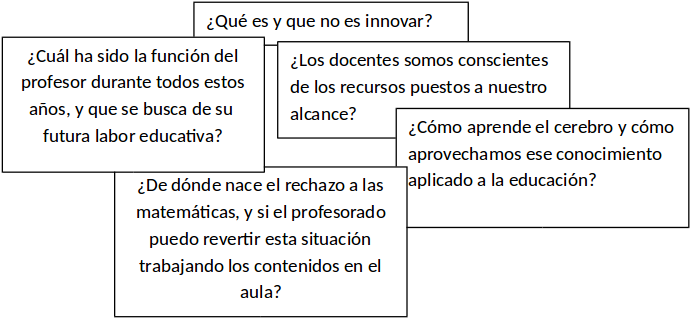
\includegraphics[scale=0.5]{img/pedro2.png}
%\captionof{figure}{...}
\end{minipage}

Continuando un poco en la línea, y finalizando el Tema 2, afirmamos que resulta necesario vincular las emociones al aprendizaje. La única manera de lograr este hecho es mediante la utilización de recursos apropiados por parte del profesorado para captar la atención del alumnado. Para corroborar esta afirmación cito una frase: “La atención no se presta, se capta” (Javier Espinosa, jornada de Gamificación). Actualmente esta emoción resulta difícil debido a la obligatoriedad de las matemáticas, por eso tenemos que buscar la manera de divulgar los contenidos para lograr que el alumno sienta la curiosidad por descubrir.

 
Llegado este punto, me cuestiono mi labor como educador. ¿Tengo que limitarme a mis obligaciones como mero transmisor de conocimiento matemáticos, o tengo que hacer un esfuerzo de divulgación para sacar a la luz su verdadera utilidad?

\textbf{A medida que avanza la clase, saco mi propia conclusión.}

Tengo que ser capaz de enseñar competencias claves a mis alumnos, y para ello buscar la mejor forma de hacerlo utilizando diferentes recursos. De esta manera, lograré que ellos tomen conciencia de la utilidad de las matemáticas:

\begin{center}
\textbf{“HACER QUE LOS ALUMNOS PIENSEN SIN TENER CONCIENCIA DE ELLO”}
\end{center}

 Destacamos “divulgaMAT”, web de divulgación matemática con gran cantidad de recursos educativos, página que en un futuro me reportará ayuda para captar la atención del alumnado a través de actividades.

No hay que dejar pasar por alto el daño matemático que en ocasiones hacen los medios de comunicación. Hay casos en los que no se utilizan las matemáticas como una herramienta, sino que la manipulan para que nos creamos la información (Web curiosa sobre fallos matemáticos: malaprensa.com). En el otro extremo tenemos grandes aportes a las matemáticas en los medios, como por ejemplo las series “Universo Matemático” y “Más por menos” o el programa  “Orbita Laika”, entre otros.

Un buen divulgador matemático debe utilizar buenos ejemplos para mejorar la comprensión por parte de los alumnos, consiguiendo forjar un aprendizaje duradero. Es muy enriquecedor divulgar nuestros logros educativos, para que otros alumnos puedan beneficiarse de nuestros avances, creando una red de recursos cada vez mayor. (Objetivo de “divulgaMAT”)

\subsubsection{Jornada de formación complementaria: \textsc{Taller de Gamificación} con Javier Espinosa - 27/10/2016}

\begin{minipage}[hbtp]{1.0\linewidth}
\centering
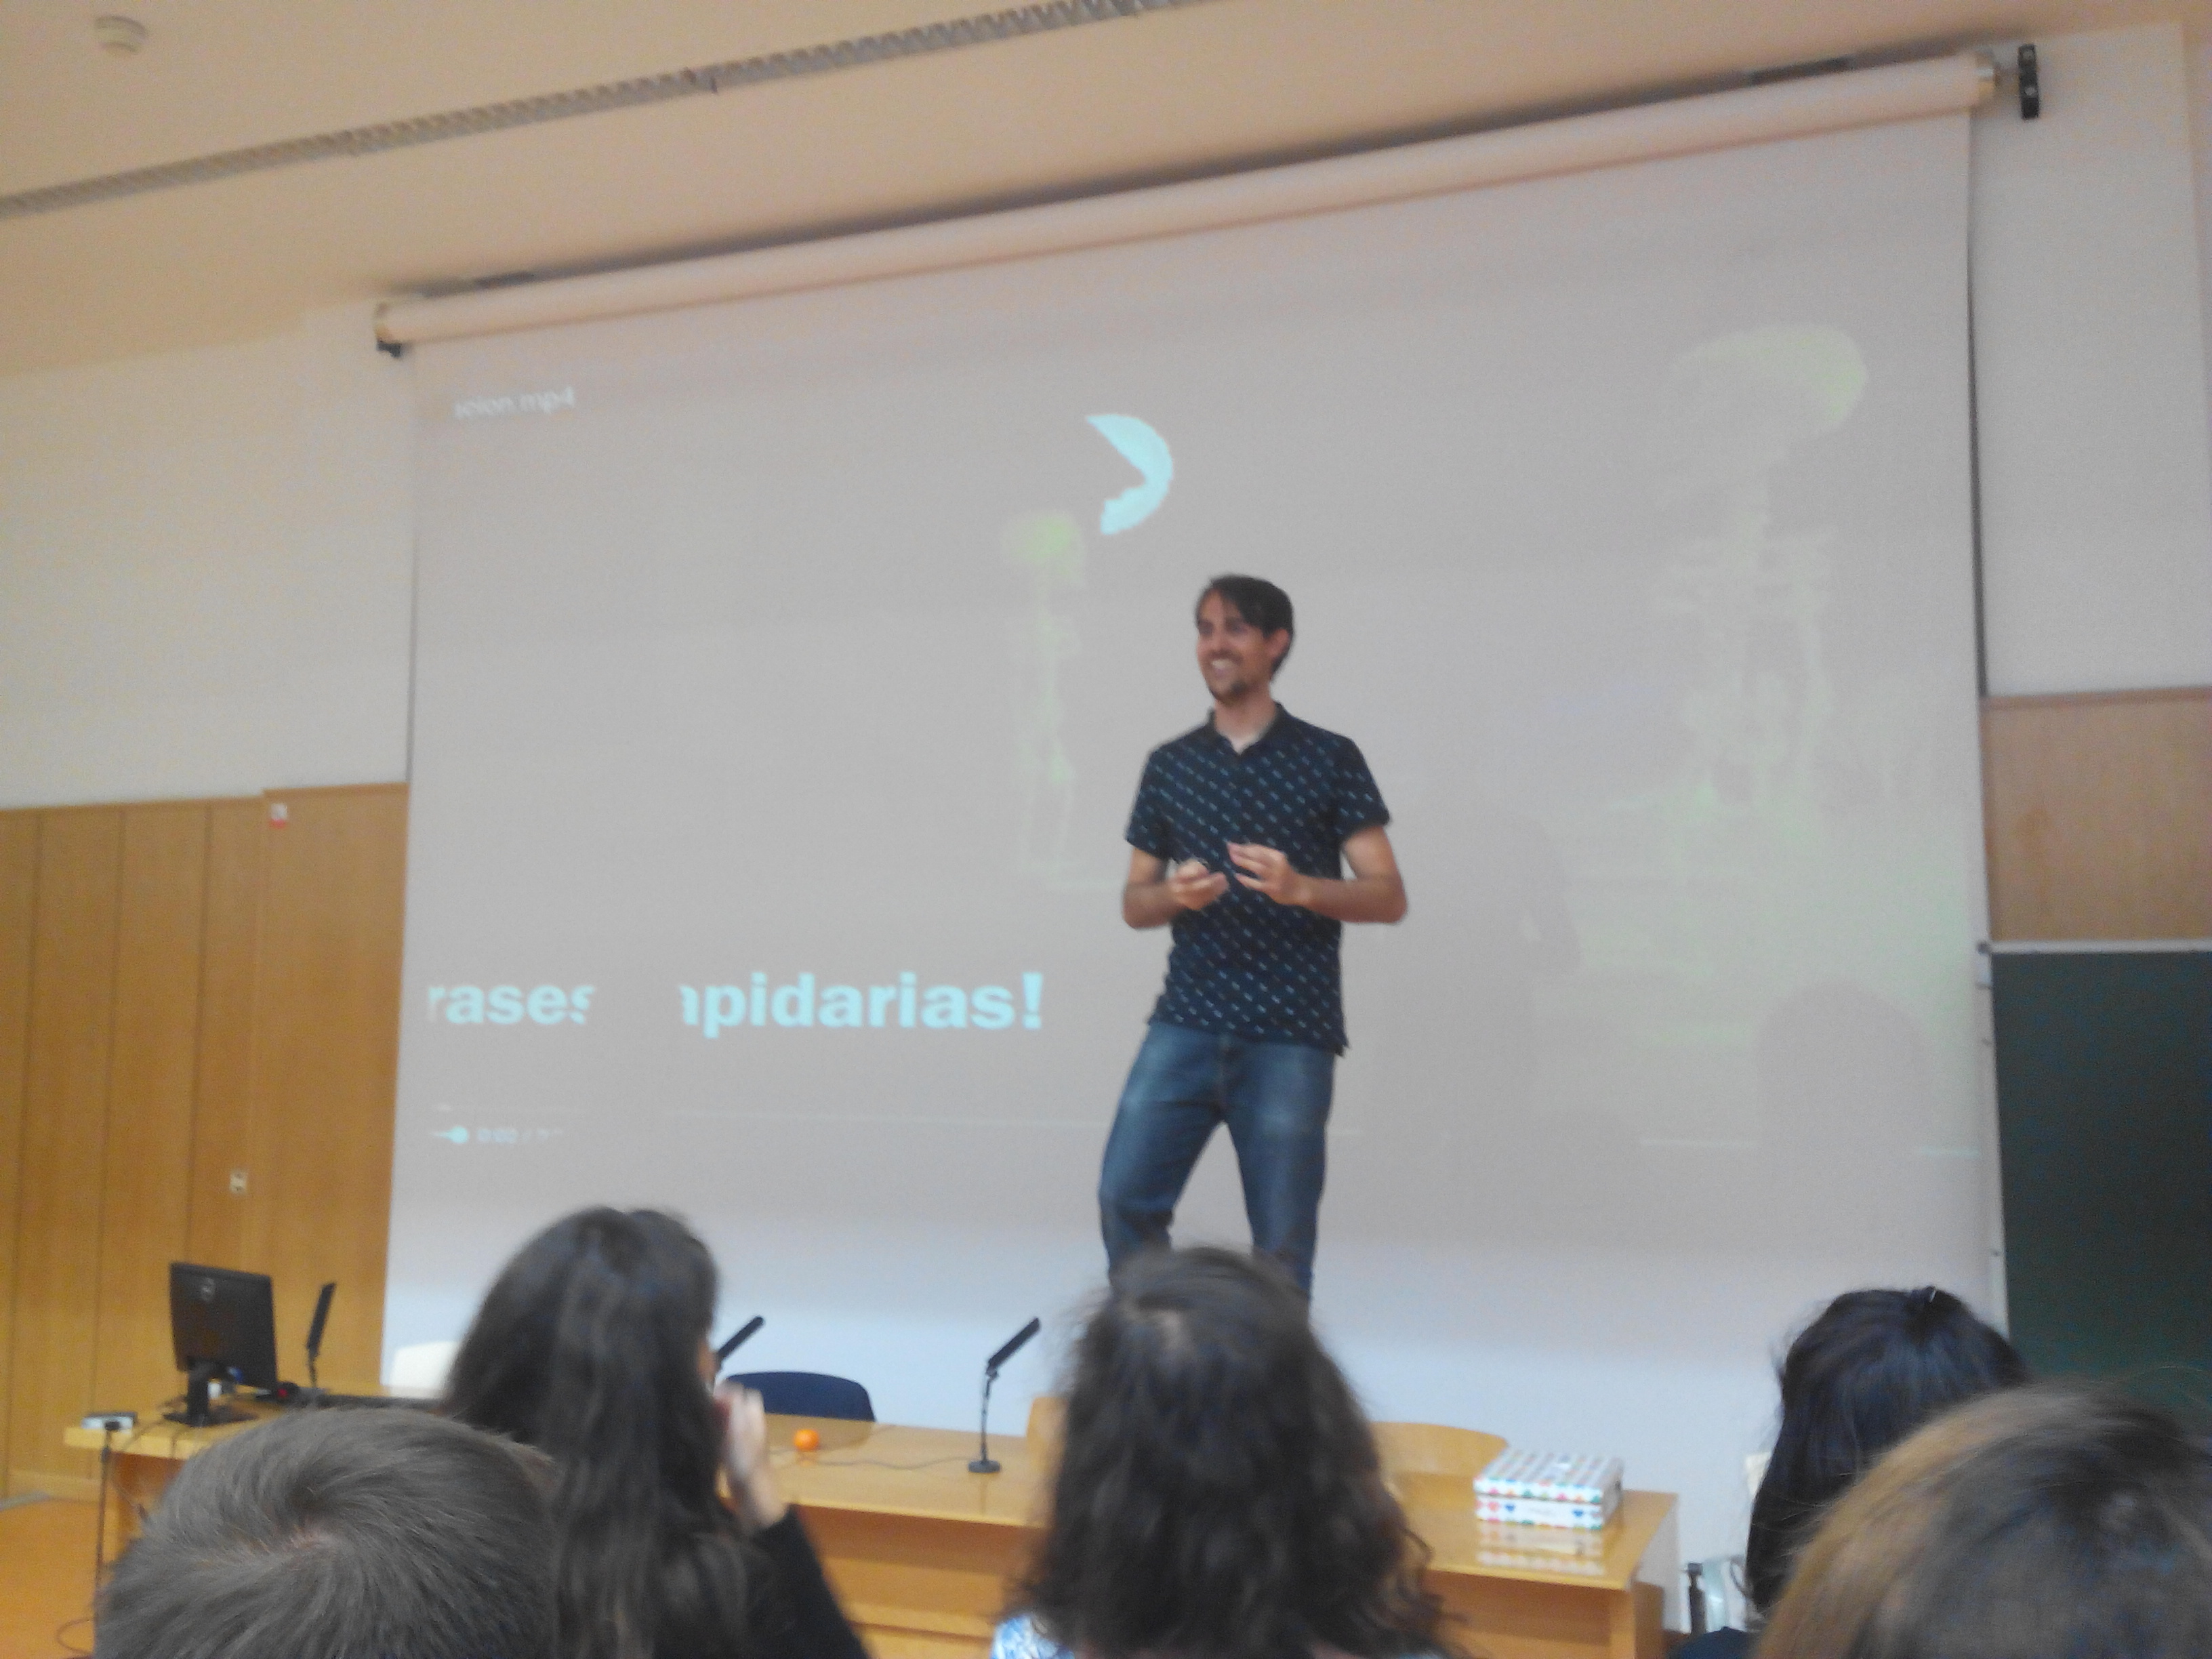
\includegraphics[scale=0.1]{img/gamingpedro.jpg}
\captionof{figure}{Jabier Espinosa al comienzo de la Jornada de Formación.}
\end{minipage}

Javier fue capaz de mantenernos  sin parpadear durante dos horas. Bailamos, reímos  y aprendimos. Comenzó la ponencia con un formulario vía Google Forms para romper el hielo, muy buena idea para un primer día de clase.

Nos pidió que fuéramos “HACKERS” del sistema, como nuevos docentes tendremos que ser capaces de buscar los recursos necesarios para mejorar la educación. La principal forma de conseguirlo es cambiar de “PASIOFF” a “PASION” en nuestro interruptor de educador. “UN SIMPLE CLICK”

Recalcó que no todos íbamos a tener unos buenos comienzos en este mundillo, pero que debemos evitar guiarnos por esos pensamientos que minan nuestra moral y buscar la manera de captar la atención de nuestros alumnos. Javier logró ganarse a sus alumnos emocionándolos mediante el empleo de la gamificación.

Dejó bien claro el concepto de gamificación, no debemos confundirlo con el termino juego. El juego no tiene un fin concreto, mientras que la gamificación implica un proceso creado por el profesor con un fin didáctico.

Aquí es donde Javier nos invitó a crear una experiencia siguiendo una serie de pautas:

\begin{itemize}

\item En primer lugar analizar el aula, identificando los diferentes tipos de jugadores: 

\begin{minipage}[hbtp]{1.0\linewidth}
\centering
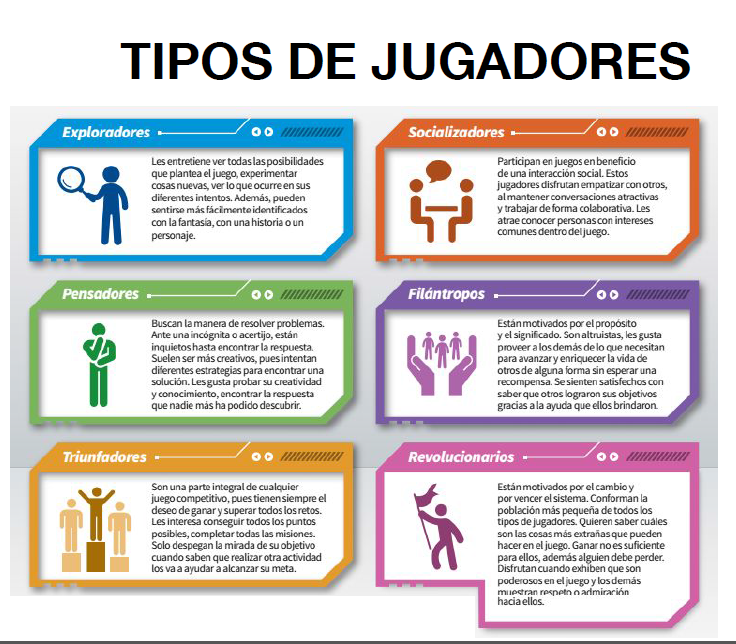
\includegraphics[scale=0.45]{img/gamingpedro2.png}
\captionof{figure}{Tipos básicos de jugadores en la gamificación.}
\end{minipage}

\item Crea tu propia historia dando rienda suelta a tu creatividad, pero hay que ser cauteloso para no perder de vista los objetivos didácticos del juego. No siempre las historias que requieren más esfuerzo por parte del profesorado tienen una mayor aceptación entre el alumnado, así que no malgastes tus fuerzas innecesariamente. 

\item Tabla de clasificación de los alumnos, es muy importante que ellos vean su progreso en la actividad. 

\begin{minipage}[hbtp]{1.0\linewidth}
\centering
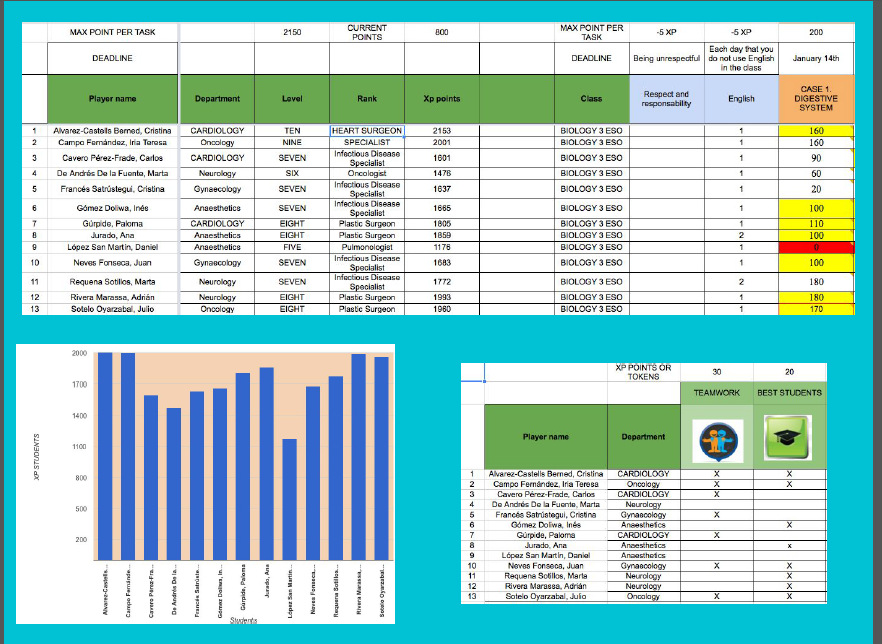
\includegraphics[scale=0.35]{img/gamingpedro3.png}
\captionof{figure}{\textit{Scoreboard} de la clase o cuaderno de notas del profesor.}
\end{minipage}

\item Crear diferentes niveles, para que los alumnos vayan progresando con sus logros. 

\begin{minipage}[hbtp]{1.0\linewidth}
\centering
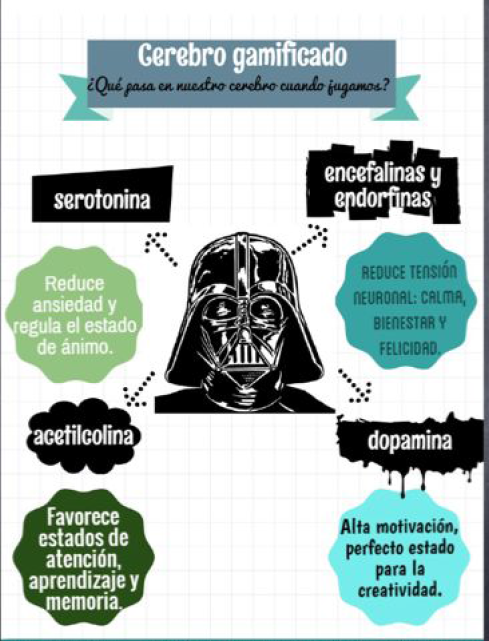
\includegraphics[scale=0.55]{img/gamingpedro4.png}
%\captionof{figure}{...}
\end{minipage}
\end{itemize}


La mejor manera de comprobar el gran trabajo realizada por Javier, es darse una vuelta por su blog \url{http://gamificationspain.weebly.com/blog/mis-gamificaciones-ah-las-tenis} . En él nos habla de sus dos proyectos de gamificación:

\begin{itemize}

\item \textbf{\textsc{Earthxodus}}: Una aventura apocalíptica para 1º de la ESO en la asignatura de Naturales. Donde los alumnos tiene que recorrer el planeta estudiando la atmósfera, hidrosfera y geosfera. Incorpora una tienda donde intercambiar su dinero virtual (tokens) por tickets especiales. Todo adaptado al contenido curricular de la asignatura. El enlace es \url{iaravaca.wix.com/1eso}

\item \textbf{\textsc{The Hospital}}: Un hospital donde llegan casos de famosos y los alumnos son médicos que les tienen que curar a la vez que estudian anatomía. Desde Miley Cyrus con un problema digestivo hasta Lady Gaga con problemas respiratorios. El enlace es \url{iaravaca.wix.com/thehospital} 

\end{itemize}

\end{opin}

\begin{opin}{\virgicolor}{Virginia}

En el siguiente punto, se analiza por tanto la relación fundamental que existe entre \textbf{las emociones y el aprendizaje}.  Francisco Mora dice que las emociones son la base más importante sobre la que se sustentan todos los procesos de aprendizaje y memoria. Estoy completamente de acuerdo ya que a veces no nos acordamos lo que hicimos ayer y sin embargo recordamos algo que pasó años atrás por el simple hecho de que lo asociamos a un momento emocional. Por ejemplo, Raquel nos preguntó que estábamos haciendo el 11 de Septiembre de 2011 y enseguida me vino a la memoria lo que hice porque lo asocie a la tragedia de las torres gemelas. La cuestión es emocionarse independientemente de que sea por algo negativo como es el caso de las torres gemelas como si es por algo positivo. En este caso, recuerdo perfectamente lo que estaba haciendo el día que me enteré que había conseguido el trabajo que tengo actualmente. Por tanto, puesto que en nuestra vida personal los recuerdos los asociamos con las emociones y los retenemos mucho mejor, parece evidente que sí conseguimos que los alumnos se emocionen con aquello que están aprendiendo, el proceso de aprendizaje será más efectivo y los conocimientos que adquieran serán más duraderos.

Encontré una entrevista que se le hace a Francisco Mora en la 2 de TVE que me resultó muy interesante en las que destaca que \textit{“para aprender hay que evocar curiosidad”} y que \textit{“no hay razón sin emoción”.}

\url{http://www.rtve.es/alacarta/videos/para-todos-la-2/para-todos-2-entrevista-francisco-mora-aprender/1840491/}

La labor del profesor es fundamental en este sentido. Es decir, tenemos que hacer que los alumnos se emocionen con aquello que explicamos, hay que ser capaces de motivarles, manteniendo su curiosidad. Tenemos que conseguir que vean el aprendizaje como algo divertido ya que cuando nos divertimos el cuerpo segrega dopamina que activa el circuito cerebral y provoca “ganas de más”. En el blog de escuela con cerebro me gustó mucho cómo un grupo de alumnos hicieron una animación sobre un problema de física (ver Figura \ref{playmovil}). Estoy segura que al realizar la animación, se divirtieron, segregaron dopamina, y consiguieron establecer una conexión entre las emociones que sintieron al realizar el juego de animación y el aprendizaje del problema de física, afianzando de forma más duradera los nuevos conocimientos de física adquiridos.



\begin{minipage}[hbtp]{1.0\linewidth}
\centering
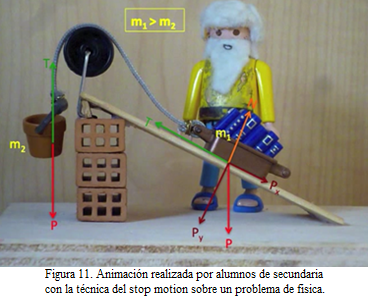
\includegraphics[scale=0.8]{img/playmovil.jpg}
\captionof{figure}{Animación realizada por alumnos de secundaria sobre un problema de física}
\label{playmovil}
\end{minipage}


Otro artículo importante de este blog es el de “Motivación escolar: siete etapas clave”. Las etapas clave son las siguientes:

\begin{itemize}

\item Qué curioso: hay que provocar curiosidad. 

\item Esto me interesa: demostrar que lo que se enseña es útil. 

\item Acepto el reto: no puede ser algo muy sencillo porque provocará aburrimiento ni algo demasiado complicado porque provocaría desmotivación y es lo contrario a lo que se busca. 

\item Soy el protagonista: el alumno tiene que ser un participante activo en el aprendizaje para que se sienta importante en dicho proceso. 

\item Progreso: es importante que el alumno se sienta valorado por su esfuerzo y que se cree un clima emocional positivo en la clase. 

\item Esto vale la pena: promover la autoevaluación para que el alumno se dé cuenta que su progreso es efectivo y sirve para algo. 

\item Soy útil: promover el trabajo cooperativo de forma que se muestre que cada participante del grupo es esencial en la consecución del objetivo del grupo en su conjunto. 
\end{itemize}

\end{opin}
